\begin{scanpage}{0077}{60}
By means of equation
\[\begin{gathered}H_0^{(1)}(qD)=\frac1{i\pi}\int_{-\infty}^{\infty}\frac{e^{ip\sqrt{D^2+\zeta^2}}}{\sqrt{D^2+\zeta^2}}e^{-it\zeta}\,d\zeta,\\q=\sqrt{p^2-t^2},\quad\operatorname{Im}q>0,\quad D>0,\end{gathered}\tag{11.11}\]
which follows from Equation (3.10), if one substitutes $z=t$, $w=\zeta$, $d=-ip$, $k=-iD$, in it we find that
\[\mathbf A=\frac{i\pi}c e^{ikx_1\cos\alpha_1}\int_{-\infty}^a\mathbf J(\eta)H_0^{(1)}\left(k\sqrt{z^2+(y_1-\eta)^2}\right)e^{ik\eta_1\cos\beta_1}\,d\eta.\tag{11.12}\]
\begin{minipage}[t]{.43\linewidth}\vspace{0pt}\centering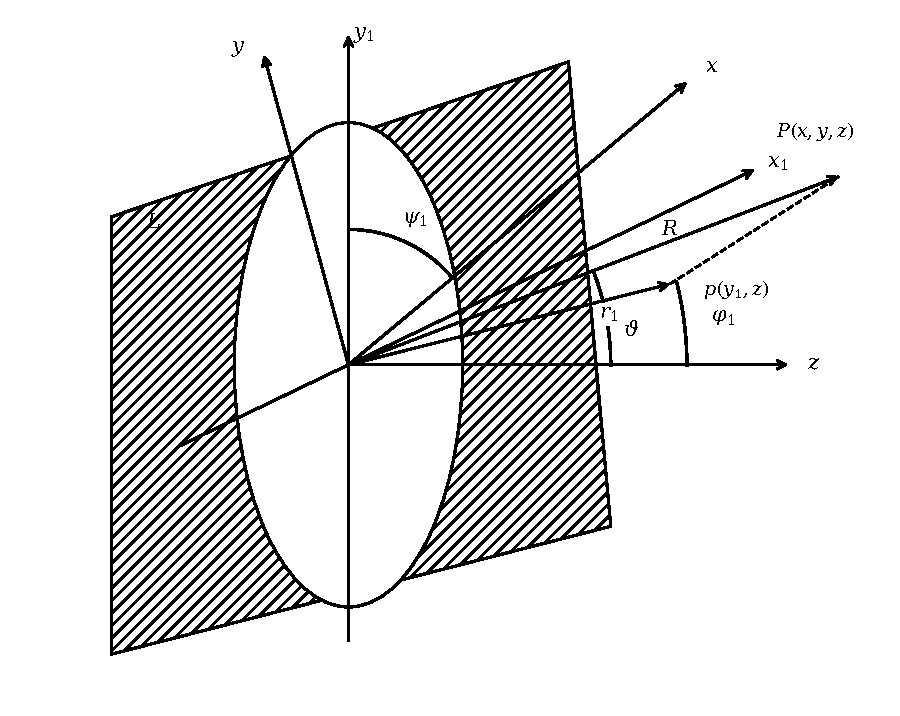
\includegraphics[width=.95\linewidth]{images/recreated/a-0077-fig23.pdf}\par Figure 23. Diffraction by a disk with oblique incidence of a plane wave. The half-plane $L$ lies in the plane of the disk. Its edge is tangent to the circumference of the disk at the point $x_1=0$, $y_1=a$ ($a$ is the radius of the disk).\end{minipage}\hfill\begin{minipage}[t]{.53\linewidth}\vspace{0pt}
Taking the fact into account that the nonuniform part of the current is concentrated mainly in the vicinity of the half-plane edge and using the asymptotic representation of the Hankel function, we obtain
\end{minipage}
\[\mathbf A=\frac1c\sqrt{\frac{2\pi}{k_1r_1}}e^{ik(x_1\cos\alpha_1+r_1\sin\alpha_1)+i\frac\pi4}\int_{-\infty}^a\mathbf J(\eta)e^{ik\eta_1\Phi_1}\,d\eta,\tag{11.13}\]
where
\[\begin{aligned}\Phi_1&=\cos\beta_1-\sin\alpha_1\sin\phi_1=\\&=\sin\gamma\sin\psi_1-\sin\theta\cos(\psi_1-\phi)\sqrt{\frac{1-\sin^2\gamma\cos^2\psi_1}{1-\sin^2\theta\sin^2(\psi_1-\phi)}}.\end{aligned}\tag{11.14}\]
In the case when $\psi_1=\delta$ [see Equations (11.04) and (11.05)] the function $\Phi_1$ takes the value
\[\Phi_1=-\sqrt{\lambda^2+\mu^2}.\tag{11.15}\]
Starting from expression (11.13), it is not difficult to show that the fringing field in the far zone is described by the following equations:
\end{scanpage}
